\subsection{Use Case}
\begin{figure}[H]
\label{fig:uc3}
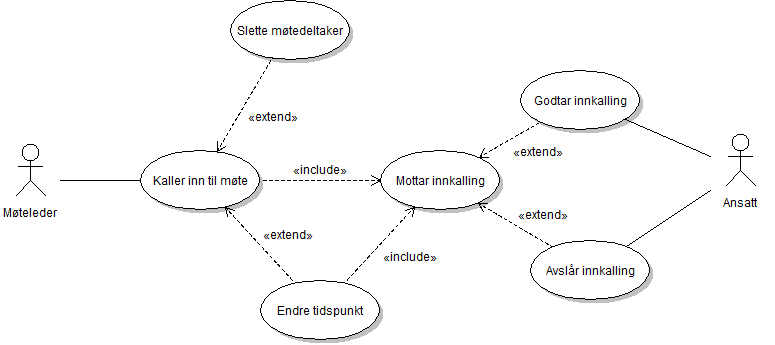
\includegraphics[width=400px]{ucs3.png}
\caption{Use Case-diagram for scenario 3}
\end{figure}

\subsection{Tekstlig Use Case}
\begin{table}[H]
\centering
\label{tab:tuc3}
\begin{tabular}{| l | L{4in} |}
\hline
Use Case & Scenario 3 \\
\hline
Aktør & Møteleder og inviterte ansatte \\
\hline
Trigger & Møteleder inkaller til møte \\
\hline
Pre-betingelser & Brukerene må være logget inn og invitert til samme møte. \\
\hline
Post-betingelser & Møtet blir satt hvor brukerene som har godtatt er invitert og de som har avlyst blir slettet fra møteinkallelsen. \\
\hline
Normal hendelsesflyt & 
\begin{minipage}{4in}
\vskip 4pt
\begin{itemize}
\item Møteleder inkaller til møte
\item Inviterte ansatte mottar møteinkallelse
\item Noen akspeterer møteinkalleslsen og noen avslår møteinkallelsen
\end{itemize}
\vskip 4pt
\end{minipage}
 \\
\hline
Variasjoner & 
\begin{minipage}{4in}
\vskip 4pt
\begin{itemize}
\item Møte blir planlagt på nytt
\item De som avslår møteinkallelsen blir slettet fra møteinkallelsen
\end{itemize}
\vskip 4pt
\end{minipage}
\\
\hline
Relatert informasjon & Alle ansatte som er invitert får beskjed om endringer som blir gjort i møteinkallelsen. \\
\hline
\end{tabular}
\caption{Tekslig Use Case-diagrame}
\end{table}

\subsection{Sekvensdiagram}
\begin{figure}[H]
\label{fig:sek3}
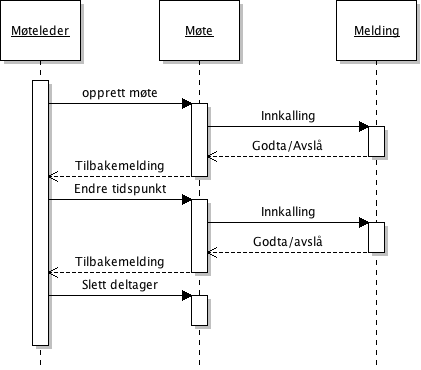
\includegraphics[width=400px]{sekvens3.png}
\caption{Use Case-diagram for scenario 3}
\end{figure}